\documentclass[11pt,a4paper,french,twoside]{PMCours}
\usepackage{hyperref}
\usepackage{lastpage}
\frenchbsetup{StandardLists=true}

\begin{document}
\TitreISN{Classe de Terminale}{Année 2021--2022}
{Numérique et Sciences Informatiques}{Épreuve de Spécialité - Sujet 2 - 3h30}

\medskip
{\large Dès que ce sujet vous est remis, assurez-vous qu’il est complet.
\textbf{Ce sujet comporte \pageref{LastPage} pages.}

\medskip
Chaque candidat traitera trois exercices au choix parmi les cinq proposés, 
chaque exercice étant noté sur sept points.

\medskip
\textbf{Les exercices seront rendus sur des copies séparées.}

\medskip
L'usage de tout document, calculatrice, etc... est interdit.

\medskip
\textbf{Les élèves rendront de manière impérative brouillons et sujet en même temps que leur composition.}}

\newpage
\section*{Exercice 1}
\emph{Cet exercice porte sur les bases de données relationnelles et le langage SQL}

\medskip
Cet exercice utilise les mots du langage SQL parmi :
\begin{verbatim}
SELECT, FROM, WHERE, JOIN, ON, INSERT INTO, DELETE FROM, 
VALUES, ORDER BY, ASC, DESC, DISTINCT, AS,
LIMIT, LIKE, IN, AND, OR, NOT, MIN, MAX, COUNT, SUM,
<, >, <=, >=, =, !=
\end{verbatim} 
\ \\
On rappelle que :
\begin{itemize}
\item \code{DISTINCT} utilisé après \code{SELECT} supprime les doublons dans les résultats des requêtes.
\item \verb'ORDER BY' permet de classer les résultats d'une requête (par ordre croissant \code{ASC} ou décroissant \code{DESC}) et obéit à la syntaxe : 
\begin{verbatim}
SELECT Attributs FROM Table WHERE Condition ORDER BY Attribut_de_classement ASC (ou DESC)
\end{verbatim}
\item \code{COUNT} renvoie le nombre de lignes dans la réponse à une requête et obéit à la syntaxe :
\begin{verbatim}
SELECT COUNT(Attribut) FROM Table WHERE Condition
\end{verbatim}
\item \code{MIN}, \code{MAX}, \code{SUM} s'utilisent de manière similaire.
\end{itemize}

%On rappelle que \verb's LIKE m', où \verb's' est le nom d'un attribut de type chaîne de caractères et \verb'm' est un motif de chaîne de caractères (contenant le caractère \verb"'_'" qui remplace n'importe quel caractère ou bien le caractère \verb"'%'" qui remplace n'importe quelle chaîne de caractères), renvoie un booléen indiquant si \verb's' est compatible avec le motif \verb'm'. Par exemple, \verb'"Bonjour" LIKE "B_nj%"' renvoie \verb'true'.
\ \\
Les types SQL des attributs utilisés dans cet exercice sont : 
\begin{verbatim}
Int, Float, String, Time, Date, Boolean
\end{verbatim} 
Le format retenu pour le type \verb'Time' est JJ/MM/AAAA (sans guillemets) et 
le format retenu pour le type \verb'Date' est HH:MM (sans guillemets).

\medskip
Un ingénieur en informatique doit concevoir une base de données relationnelle pour gérer l'aéroport de Lesquin. Cette base de données sert pour l'affichage des informations de vols que les voyageurs peuvent consulter, ainsi qu'aux mécaniciens chargés des opérations de maintenance. Pour cela, il envisage quatre relations, dont des extraits sont précisés ci-après. Les attributs soulignés d'une relation désignent la clé primaire. Les attributs suivis du symbole \verb'#' désignent des clés étrangères.

\begin{itemize}
\item \verb'Compagnie' (Nom : String, \underline{Symbole} : String, CodePays : String)
\begin{figure}[ht]
\begin{center}
\begin{tabular}{|c|c|c|}\hline
Nom & Symbole & CodePays\\\hline
Air France & AF & F\\\hline
Air Toto & AT & F\\\hline
Sky Freedom & SKF & GB\\\hline
\end{tabular}
\end{center}
\caption{Extrait de la relation \textbf{Compagnie}}
\end{figure}
\end{itemize}

\begin{itemize}
\item \verb'Avion' (\underline{RefComp} \verb'#' : String, \underline{Matricule} : String, Modele : String, RayonDActionKm : Float, VitesseMaxKmH : Float, NbDePassagers : Int)
\begin{figure}[ht]
\begin{center}
\begin{tabular}{|c|c|c|c|c|c|}\hline
RefComp & Matricule & Modele & RayonDActionKm & VitesseMaxKmH & NbDePassagers\\\hline
AF & AF 1234 & Airbus A380 & 2500 & 780 & 550\\\hline
SKF & SKF 547 & Boeing 737 & 1500 & 974,8 & 350\\\hline
LFT & LFT 78549 & Airbus A350 & 1700,5 & 830,0 & 350\\\hline
\end{tabular}
\end{center}
\caption{Extrait de la relation \textbf{Avion}}
\end{figure}
\end{itemize}

\begin{itemize}
\item \verb'Vol' \\
\begin{figure}[ht]
\begin{center}
\begin{tabular}{|c|c|c|c|c|c|}\hline
Reference & Type & Date & Horaire & Lieu & Retard\\\hline
SKF 547 & Départ & 14/07/2022 & 14:30 & Londres & false\\\hline
LFT 78549 & Arrivée & 12/06/2022 & 13:00 & Paris & true\\\hline
LFT 78549 & Départ & 16/08/2022 & 07:15 & Berlin & false\\\hline
\end{tabular}
\end{center}
\caption{Extrait de la relation \textbf{Vol}}
\end{figure}
Le lieu d'un vol de type 'Départ' désigne l'aéroport de destination de ce vol. Le lieu d'un vol de type 'Arrivée' désigne l'aéroport de provenance de ce vol. 
\end{itemize}

\begin{itemize}
\item \verb'Operation' (\underline{Reference} \verb'#' : String, \underline{Date} : String, Horaire : Time, HoraireFin : Time, Nature : String)
\begin{figure}[ht]
\begin{center}
\begin{tabular}{|c|c|c|c|c|}\hline
Reference & Date & HoraireDebut & HoraireFin & Nature\\\hline
LFT 78549 & 17/06/2022 & 10:15 & 15:00 & Visite mensuelle des moteurs\\\hline
AF 1234 & 17/06/2022 & 09:00 & 13:00 & Réparation volet droit\\\hline
AF 1234 & 01/05/2022 & 08:00 & 17:00 & Visite annuelle générale\\\hline
\end{tabular}
\end{center}
\caption{Extrait de la relation \textbf{Operation}}
\end{figure}
\end{itemize}

\begin{enumerate}
\item Écrire le schéma relationnel de la table \verb'Vol' (sans préciser de clé primaire), en indiquant les éventuelles clés étrangères.
\item Pourquoi l'attribut \verb'Reference' ne peut pas être utilisé comme clé primaire pour la relation \verb'Vol' ? Proposez une clé primaire valide, avec le minimum d'attributs, sachant qu'un avion peut faire plusieurs rotations par jour vers une même destination.
\item Avec cette base de données, un avion peut-il avoir plusieurs opérations de maintenance le même jour ? Justifier.
\item Qu'affiche la requête SQL suivante :
\begin{verbatim}
SELECT Reference FROM Operation WHERE Date = 17/06/2022 AND HoraireFin >= 14:00
\end{verbatim} 
\item Écrire une requête SQL qui affiche la référence des vols retardés le 28 Janvier 2022.
\item Écrire une requête SQL qui ajoute à la relation \verb'Avion' l'Airbus A321, de matricule SKF 2468, dont la vitesse maximale est de 960 km/h, pouvant emporter 260 passagers sur une distance maximale de 1800 km.
\item Écrire une requête SQL qui affiche les horaires des vols qui sont en provenance de Strasbourg le vendredi 1er avril 2022.
\item Écrire une requête SQL qui affiche le nombre de compagnies françaises (le code pays de la France étant F).
\item Écrire une requête SQL qui donne le nombre maximal de passagers qu'un modèle d'avion puisse transporter.\\
Écrire alors une requête SQL qui affiche les modèles d'avion qui peuvent transporter le plus de passagers.
%\item Ecrivez une requête SQL qui affiche le matricule des avions qui n'ont pas d'opération de maintenance prévue le mercredi 11 mai 2022, ni le mercredi 18 mai 2022.
\item On exécute la requête SQL suivante :
\begin{verbatim}
DELETE FROM Avion WHERE Matricule = "AF 1234"
\end{verbatim} 
mais un message d'erreur est renvoyé, indiquant que l'opération est impossible. Expliquer pourquoi, en analysant les extraits de la base de données fournis, puis écrivez les commandes SQL complémentaires, en plus de celle-ci, afin que la requête puisse être réalisée avec succès.
\item Écrire une requête SQL qui affiche, sans répétition, le nom des compagnies aériennes qui possèdent au moins un Airbus A350.
\item Pour des raisons logistiques, une opération de maintenance ne peut pas être programmée pour un avion un jour où il effectue un vol. Écrire une requête SQL qui affiche les matricules d'avions qui ne respecteraient pas cette règle, c'est à dire pour lesquels une opération de maintenance serait prévue un jour où ils doivent voyager. 
\item Écrire une requête SQL qui affiche la liste des couples nom de compagnie / matricule d'avion de cette compagnie, triée dans l'ordre alphabétique décroissant des noms de compagnie.
%\item Ecrivez une requête SQL qui affiche le nombre total de passagers que la compagnie aérienne Air France peut transporter avec ses avions.
% \item Ecrivez une requête SQL qui affiche les références des vols d'avions qui font escale à l'aéroport de NataSahId. Par convention, on suppose qu'un avion fait une escale lorsqu'il atterrit puis redécolle le même jour.
%\item Ecrivez une requête SQL qui affiche les matricules des avions français qui ont une visite annuelle générale prévue en janvier 2022.
\item Écrire une requête SQL qui affiche le modèle de tous les avions qui arrivent de Londres ou partent vers Londres.
\end{enumerate}


\newpage
\section*{Exercice 2}
\emph{Cet exercice porte sur les réseaux et l'architecture.}

\medskip


\subsection*{Partie 1 : Protocole RIP}
On considère le réseau suivant (chaque routeur est repéré par une lettre) :
\begin{center}
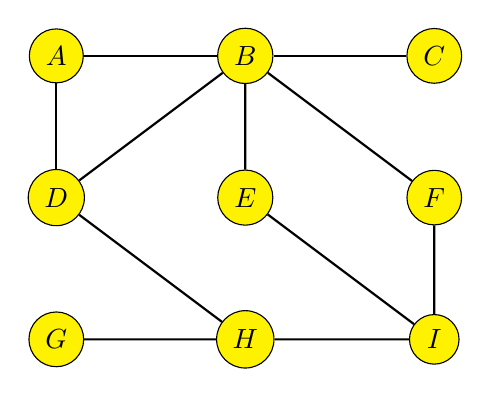
\begin{tikzpicture}[xscale=0.8,yscale=0.8]
% Styles (MODIFIABLES)
\tikzstyle{fleche}=[-,>=latex,thick]
\tikzstyle{noeud}=[fill=yellow,circle,draw]
\tikzstyle{feuille}=[fill=orange,circle,draw]
% Dimensions (MODIFIABLES)
\def\DistanceInterNiveaux{3}
\def\DistanceInterFeuilles{2}
% Dimensions calculées (NON MODIFIABLES)
\def\NiveauA{(-0)*\DistanceInterNiveaux}
\def\NiveauB{(-.75)*\DistanceInterNiveaux}
\def\NiveauC{(-1.5)*\DistanceInterNiveaux}
\def\InterFeuilles{(.75)*\DistanceInterFeuilles}
% Noeuds (MODIFIABLES : Styles et Coefficients d'InterFeuilles)
\node[noeud] (Ri) at ({(4)*\InterFeuilles},{\NiveauC}) {$I$};
\node[noeud] (Rh) at ({(2)*\InterFeuilles},{\NiveauC}) {$H$};
\node[noeud] (Rg) at ({(0)*\InterFeuilles},{\NiveauC}) {$G$};
\node[noeud] (Rf) at ({(4)*\InterFeuilles},{\NiveauB}) {$F$};
\node[noeud] (Re) at ({(2)*\InterFeuilles},{\NiveauB}) {$E$};
\node[noeud] (Rd) at ({(0)*\InterFeuilles},{\NiveauB}) {$D$};
\node[noeud] (Rc) at ({(4)*\InterFeuilles},{\NiveauA}) {$C$};
\node[noeud] (Rb) at ({(2)*\InterFeuilles},{\NiveauA}) {$B$};
\node[noeud] (Ra) at ({(0)*\InterFeuilles},{\NiveauA}) {$A$};
% Arcs (MODIFIABLES : Styles)
\draw[fleche] (Ra)--(Rb);
\draw[fleche] (Ra)--(Rd);
\draw[fleche] (Rb)--(Rc);
\draw[fleche] (Rb)--(Rd);
\draw[fleche] (Rb)--(Re);
\draw[fleche] (Rb)--(Rf);
%\draw[fleche,draw=white,double=black,very thick] (Re)--(Rf);
\draw[fleche] (Rd)--(Rh);
\draw[fleche] (Re)--(Ri);
\draw[fleche] (Rf)--(Ri);
\draw[fleche] (Rg)--(Rh);
\draw[fleche] (Rh)--(Ri);
\end{tikzpicture}
\end{center}
Pour les questions suivantes, on se place dans le cadre du protocole RIP.\\
Pour départager des chemins de même longueur, on considère qu'à chaque fois que cela était possible, les connexions ont été établies dans l'ordre alphabétique. \\
Ainsi, la liaison entre \code{A} et \code{B} a été créée avant celle entre \code{A} et \code{D},...\\
De plus, un chemin entre deux routeurs est remplacé par un autre chemin uniquement si le nouveau chemin est strictement plus court.

\begin{enumerate}
    \item Quel est le chemin de H vers C ?
    \item Quelle est la distance maximale entre deux routeurs de ce réseau ? 
    \item Recopier sur votre copie et compléter la table de routage du routeur H (sur le modèle de la table du {\bf 4)}:
    \begin{center}
        \begin{tabular}{|c|c|c|}\hline
            Destination&Routeur suivant&Distance\\ \hline
            $\vdots$ &$\vdots$&$\vdots$\\ \hline
            
        \end{tabular}
    \end{center}
    \item Une liaison directe a été ajoutée entre deux routeurs.
    La nouvelle table de routage du routeur A est alors :
    \begin{center}
        \begin{tabular}{|c|c|c|}\hline
            Destination&Routeur suivant&Distance\\ \hline
            B&B &1 \\ \hline 
            C&B &2 \\ \hline 
            D&D &1 \\ \hline 
            E&B &2 \\ \hline 
            F&B &2 \\ \hline  
            G&D &2 \\ \hline 
            H&D &2 \\ \hline
            I&D &3 \\ \hline
 \end{tabular}
    \end{center}
    Entre quels routeurs la liaison a-t-elle été ajoutée ? Justifier brièvement.
\end{enumerate}

\newpage
\subsection*{Partie 2 : Protocole OSPF}
On considère le réseau suivant (chaque routeur est repéré par une lettre) :
\begin{multicols}{2}
\begin{center}
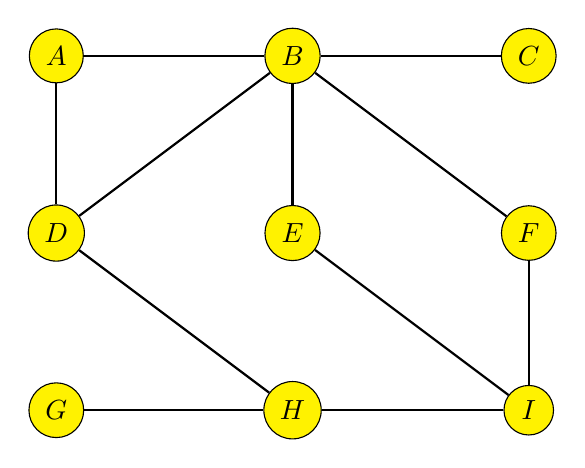
\begin{tikzpicture}[xscale=1,yscale=1]
% Styles (MODIFIABLES)
\tikzstyle{fleche}=[-,>=latex,thick]
\tikzstyle{noeud}=[fill=yellow,circle,draw]
\tikzstyle{feuille}=[fill=orange,circle,draw]
% Dimensions (MODIFIABLES)
\def\DistanceInterNiveaux{3}
\def\DistanceInterFeuilles{2}
% Dimensions calculées (NON MODIFIABLES)
\def\NiveauA{(-0)*\DistanceInterNiveaux}
\def\NiveauB{(-.75)*\DistanceInterNiveaux}
\def\NiveauC{(-1.5)*\DistanceInterNiveaux}
\def\InterFeuilles{(.75)*\DistanceInterFeuilles}
% Noeuds (MODIFIABLES : Styles et Coefficients d'InterFeuilles)
\node[noeud] (Ri) at ({(4)*\InterFeuilles},{\NiveauC}) {$I$};
\node[noeud] (Rh) at ({(2)*\InterFeuilles},{\NiveauC}) {$H$};
\node[noeud] (Rg) at ({(0)*\InterFeuilles},{\NiveauC}) {$G$};
\node[noeud] (Rf) at ({(4)*\InterFeuilles},{\NiveauB}) {$F$};
\node[noeud] (Re) at ({(2)*\InterFeuilles},{\NiveauB}) {$E$};
\node[noeud] (Rd) at ({(0)*\InterFeuilles},{\NiveauB}) {$D$};
\node[noeud] (Rc) at ({(4)*\InterFeuilles},{\NiveauA}) {$C$};
\node[noeud] (Rb) at ({(2)*\InterFeuilles},{\NiveauA}) {$B$};
\node[noeud] (Ra) at ({(0)*\InterFeuilles},{\NiveauA}) {$A$};
% Arcs (MODIFIABLES : Styles)
\draw[fleche] (Ra)--(Rb);
\draw[fleche] (Ra)--(Rd);
\draw[fleche] (Rb)--(Rc);
\draw[fleche] (Rb)--(Rd);
\draw[fleche] (Rb)--(Re);
\draw[fleche] (Rb)--(Rf);
%\draw[fleche,draw=white,double=black,very thick] (Re)--(Rf);
\draw[fleche] (Rd)--(Rh);
\draw[fleche] (Re)--(Ri);
\draw[fleche] (Rf)--(Ri);
\draw[fleche] (Rg)--(Rh);
\draw[fleche] (Rh)--(Ri);
\end{tikzpicture}
\end{center}

\begin{tabular}{|l|l|l|}\hline
    Liaison& Type   & Débit\\\hline
    A$\leftrightarrow$B&Wi-Fi&20 Mbit/s \\\hline
    A$\leftrightarrow$D&Fast Ethernet&100 Mbit/s \\\hline
    B$\leftrightarrow$C&Fibre&1 Gbit/s \\\hline
    B$\leftrightarrow$D&Ethernet&10 Mbit/s \\\hline
    B$\leftrightarrow$E&Fibre&1 Gbit/s \\\hline
    B$\leftrightarrow$F&Fast Ethernet&100 Mbit/s \\\hline
    D$\leftrightarrow$H&Fast Ethernet&100 Mbit/s \\\hline
    E$\leftrightarrow$I&Fast Ethernet&100 Mbit/s \\\hline
    F$\leftrightarrow$I&Fast Ethernet&100 Mbit/s \\\hline
    G$\leftrightarrow$H&Ethernet&20 Mbit/s \\\hline
    H$\leftrightarrow$I&Ethernet&20 Mbit/s \\\hline
\end{tabular}
\end{multicols}
Pour les questions suivantes, on se place dans le cadre du protocole OSPF.
On rappelle que pour ce protocole, le coût d'une liaison est 
$\text{coût}=\frac{10^8}{d}$ où $d$ est la bande passante en $bit/s$.
\begin{enumerate}
    \item Quel est le coût des liaisons AB et BC ? Détailler les calculs.
    \item Sans autres justifications, recopier sur votre copie le graphe et donner la pondération de chacun des arcs. 
    \item Quel est le coût total du chemin H-D-B-C ?
    \item En justifiant brièvement, quel est le chemin le moins coûteux allant de H à C ?
\end{enumerate}

\subsection*{Partie 3 : Architecture}
On s'intéresse maintenant à une station météo gérée par un Raspberry~Pi. 

Voici le schéma général du Raspberry~Pi :
\begin{center}
    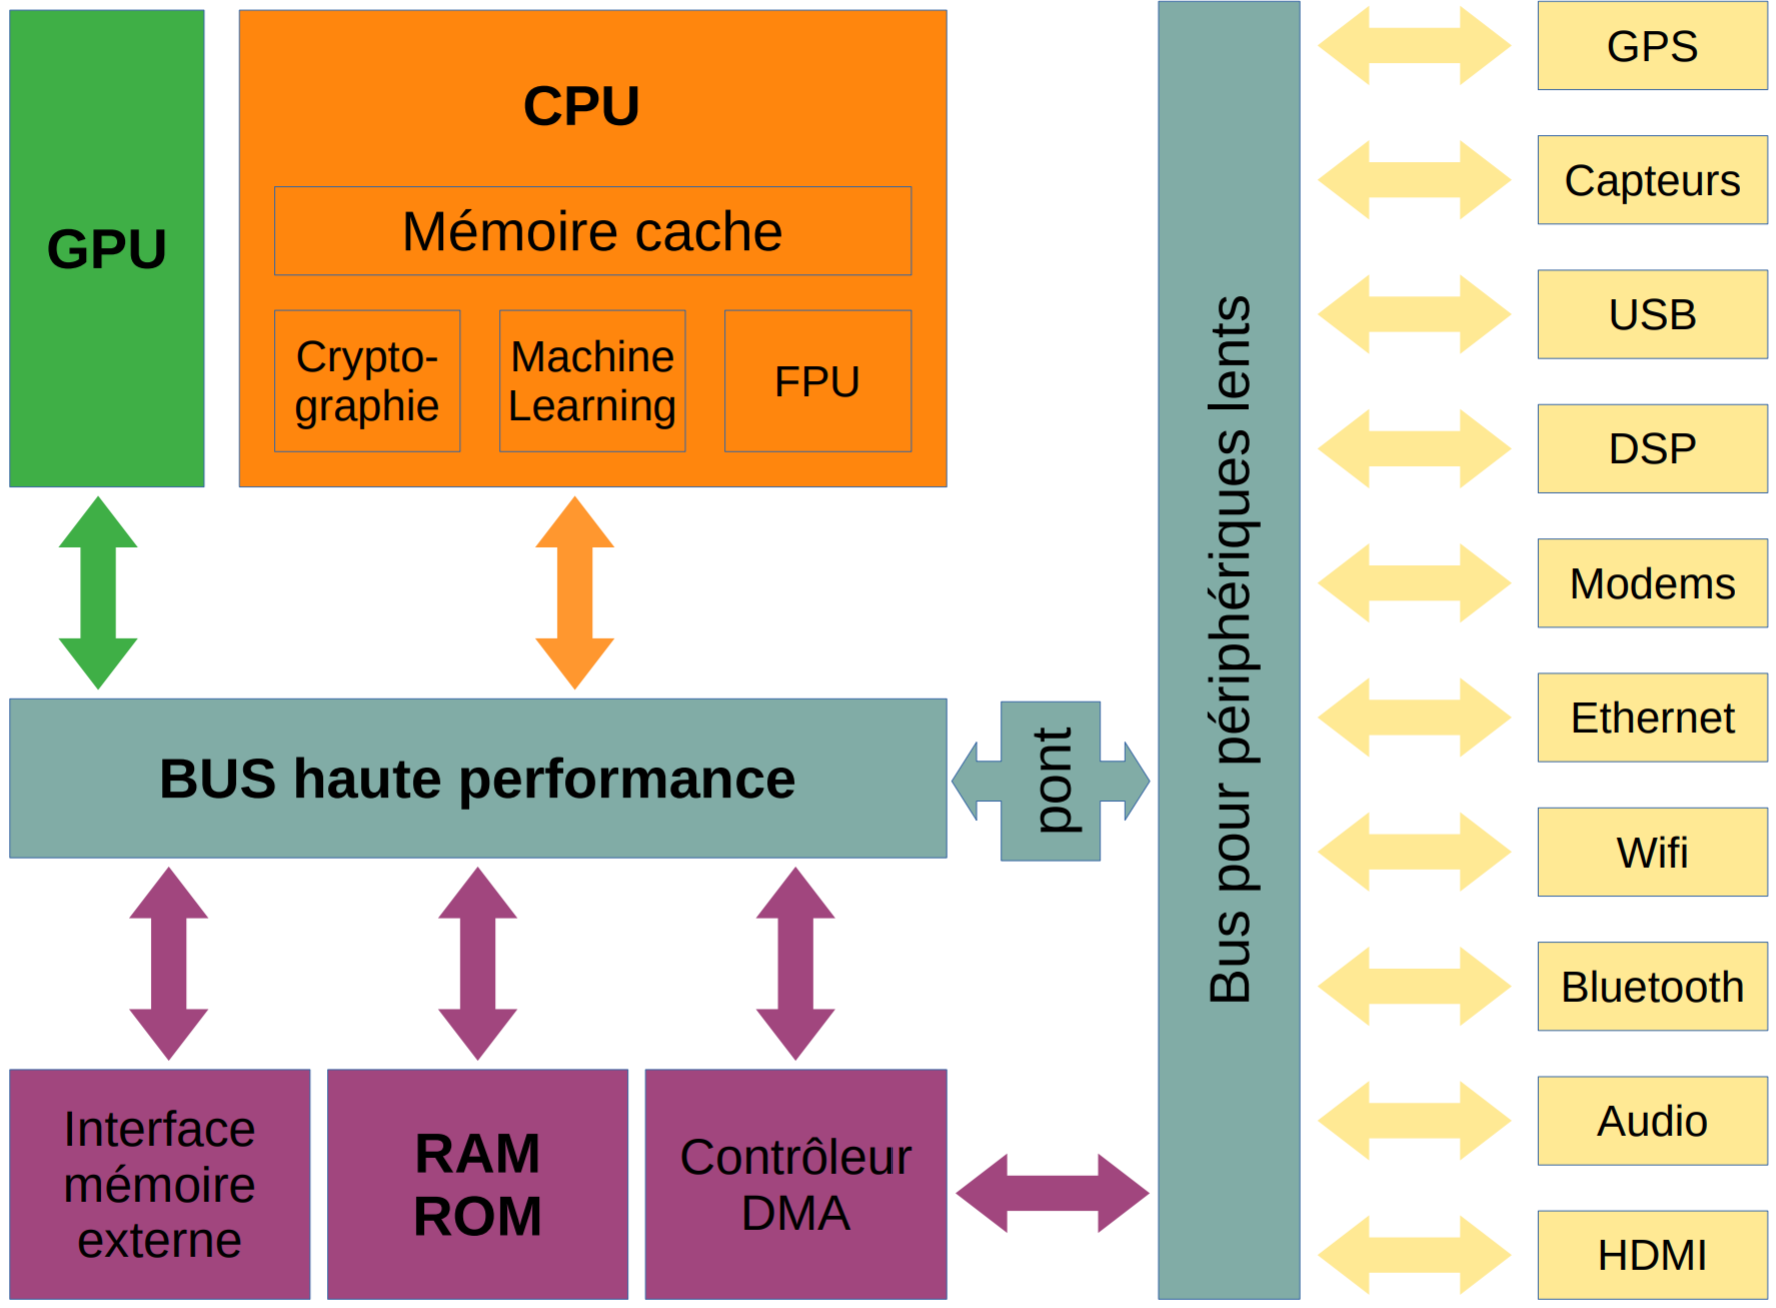
\includegraphics[width=10cm]{SchemaSoc.png}
\end{center}

Ce Raspberry~Pi est connecté au réseau internet via une liaison wifi. Il est 
relier directement avec la plupart de ses capteurs, sauf l'anémomètre à qui il 
est connecté par Bluetooth. Il dispose d'un stockage persistant grâce à un
disque SSD externe USB. Il n'a pas d'écran.  

\begin{enumerate}
    \item Donner la liste des modules d'entrée sortie (à droite dans le schéma) 
    nécessaires au bon fonctionnement de la station météo.
    \item Les processus s'exécutant sur le Raspberry~Pi ne doivent surtout pas
    s'arrêter. Expliquer ce qu'on appelle un interblocage.
\end{enumerate}


\newpage
\section*{Exercice 3}
\emph{Cet exercice traite de manipulation de tableaux, de récursivité et du paradigme
« diviser pour régner ».}

\medskip
Dans un tableau Python d'entiers \code{tab}, on dit que le couple d'indices $(i,j)$ forme une inversion
lorsque $i<j$ et \code{tab[i] > tab[j]}. On donne ci-dessous quelques exemples.
\begin{itemize}
\item Dans le tableau \code{[1, 5, 3, 7]}, le couple d'indices $(1,2)$ forme une inversion car $5 > 3$.
Par contre, le couple $(1,3)$ ne forme pas d'inversion car $5 < 7$.

Il n'y a qu'une inversion dans ce tableau.
\item Il y a trois inversions dans le tableau \code{[1, 6, 2, 7, 3]}, à savoir les couples d'indices
$(1, 2)$, $(1, 4)$ et $(3, 4)$.
\item On peut compter six inversions dans le tableau \code{[7, 6, 5, 3]} : les couples d'indices
$(0, 1)$, $(0, 2)$, $(0, 3)$, $(1, 2)$, $(1, 3)$ et $(2, 3)$.
\end{itemize}
On se propose dans cet exercice de déterminer le nombre d'inversions dans un tableau
quelconque.

\subsection*{Questions préliminaires}
\begin{enumerate}
    \item Expliquer pourquoi le couple $(1, 3)$ est une inversion dans le tableau \code{[4, 8, 3, 7]}.
    \item Justifier que le couple $(2, 3)$ n'en est pas une.
\end{enumerate}

\subsection*{Partie A : Méthode itérative}
Le but de cette partie est d'écrire une fonction itérative \code{nombre\_inversion} qui renvoie le
nombre d'inversions dans un tableau. Pour cela, on commence par écrire une fonction
\code{fonction1} qui sera ensuite utilisée pour écrire la fonction \code{nombre\_inversion}.
\begin{enumerate}
    \item On donne la fonction suivante.
\begin{Python}
def fonction1(tab, i):
    nb_elem = len(tab)
    cpt = 0
    for j in range(i+1, nb_elem):
        if tab[j] < tab[i]:
            cpt += 1
    return cpt
\end{Python}
\begin{enumerate}
\item Indiquer ce que renvoie la \code{fonction1(tab, i)} dans les cas suivants.
\begin{itemize}
\item Cas n°1 : \code{tab = [1, 5, 3, 7]} et \code{i = 0}.
\item Cas n°2 : \code{tab = [1, 5, 3, 7]} et \code{i = 1}.
\item Cas n°3 : \code{tab = [1, 5, 2, 6, 4]} et \code{i = 1}.
\end{itemize}
\item Expliquer ce que permet de déterminer cette fonction.
\end{enumerate}
\item En utilisant la fonction précédente, écrire une fonction \code{nombre\_inversion(tab)} qui
prend en argument un tableau et renvoie le nombre d'inversions dans ce tableau.

On donne ci-dessous les résultats attendus pour certains appels.
\begin{alltt}
>>> nombre\_inversions([1, 5, 7])
0
>>> nombre\_inversions([1, 6, 2, 7, 3])
3
>>> nombre\_inversions([7, 6, 5, 3])
6
\end{alltt}
\item Quelle est l'ordre de grandeur de la complexité en temps de l'algorithme obtenu ?

Aucune justification n'est attendue.
\end{enumerate}

\subsection*{Partie B : Méthode récursive}
Le but de cette partie est de concevoir une version récursive de la fonction
\code{nombre\_inversion}.

On définit pour cela des fonctions auxiliaires.
\begin{enumerate}
\item Donner le nom des algorithmes de tris que vous connaissez. \\
Parmi ceux-ci, citer un algorithme de tri ayant une complexité meilleure que quadratique.
\end{enumerate}

Dans la suite de cet exercice, on suppose qu'on dispose d'une fonction \code{tri(tab)} qui prend en
argument un tableau et renvoie un tableau contenant les mêmes éléments rangés dans l'ordre
croissant.

\begin{enumerate}\setcounter{enumi}{1}
\item Écrire une fonction \code{moitie\_gauche(tab)} qui prend en argument un tableau \code{tab} et
renvoie un nouveau tableau contenant la moitié gauche de \code{tab}. Si le nombre d'éléments
de \code{tab} est impair, l'élément du centre se trouve dans cette partie gauche.

On donne ci-dessous les résultats attendus pour certains appels.
\begin{alltt}
>>> moitie\_gauche([])
[]
>>> moitie\_gauche([4, 8, 3])
[4, 8]
>>> moitie\_gauche ([4, 8, 3, 7])
[4, 8]
\end{alltt}
\end{enumerate}

Dans la suite, on suppose qu'on dispose de la fonction \code{moitie\_droite(tab)} qui renvoie la
moitié droite sans l'élément du milieu.

\begin{enumerate}\setcounter{enumi}{2}
\item On suppose qu'une fonction \code{nb\_inv\_tab(tab1, tab2)} a été écrite. Cette fonction
renvoie le nombre d'inversions du tableau obtenu en mettant bout à bout les tableaux
\code{tab1} et \code{tab2}, à condition que \code{tab1} et \code{tab2} soient triés dans l'ordre croissant.

On donne ci-dessous deux exemples d'appel de cette fonction :
\begin{alltt}
>>> nb\_inv\_tab([3, 7, 9], [2, 10])
3
>>> nb\_inv\_tab([7, 9, 13], [7, 10, 14])
3
\end{alltt}
En utilisant la fonction \code{nb\_inv\_tab} et les questions précédentes, écrire une fonction
récursive \code{nb\_inversions\_rec(tab)} qui permet de calculer le nombre d'inversions
dans un tableau. Cette fonction renverra le même nombre que
\code{nombre\_inversions(tab)} de la partie A. On procédera de la façon suivante :
\begin{itemize}
\item Séparer le tableau en deux tableaux de tailles égales (à une unité près).
\item Appeler récursivement la fonction \code{nb\_inversions\_rec} pour compter le nombre
d'inversions dans chacun des deux tableaux.
\item Trier les deux tableaux (on rappelle qu'une fonction de tri est déjà définie).
\item Ajouter au nombre d'inversions précédemment comptées le nombre renvoyé par la
fonction \code{nb\_inv\_tab} avec pour arguments les deux tableaux triés.
\end{itemize}
\end{enumerate}

\newpage
\section*{Exercice 4}

\emph{Cet exercice porte sur les arbres et la programmation orientée objet.}

\medskip
Un concessionnaire automobile développe un programme pour gérer les véhicules qu'il
propose à la vente.

Dans ce programme, pour modéliser les données de véhicules, on définit une classe
\code{Veh} avec les attributs suivants :
\begin{itemize}
\item \code{ma} de type \code{str} représente la marque du véhicule (Peugeot, Renaut, Porsche, … ) ;
\item \code{prx} de type \code{float} est le prix à neuf du bien ;
\item \code{age} de type \code{int} est l'age du véhicule.
\end{itemize}

La classe \code{Veh} possède une méthode \code{estim\_prix} qui renvoie une estimation du prix du
véhicule. Le code (incomplet) de la classe \code{Veh} est donné ci-dessous :
\begin{Python*}
class Veh:
    def __init__(self, marque, prix_neuf, age):
        ...
    def estim_prix(self):
        return self.prx * (1-self.age/10)
\end{Python*}
Ainsi, on estime le prix d'un véhicule en enlevant $10\%$ de son prix neuf par année de circulation.
\begin{enumerate}
\item Recopier et compléter le code du constructeur de la classe \code{Veh}.
\item On exécute l'instruction suivante :

\medskip
\code{v1 = Veh('Peugeot', 10000, 4)}

Que renvoie l'instruction v1.estim\_prix() ? 
\item On souhaite affiner l'estimation du prix d'un véhicule en tenant compte de sa marque :
\begin{itemize}
\item pour un véhicule dont l'attribut \code{ma} est \code{'Peugeot'} la nouvelle estimation du prix est son prix neuf auquel on enlève 20$\%$ par année de circulation. Si le prix atteint $0$ euros, on le fixe à 1 euro. 
\item pour un véhicule dont l'attribut \code{ma} est \code{'Porsche'} la nouvelle estimation du prix est son prix neuf auquel on ajoute 10$\%$ par année de circulation; 
\item pour les biens d'autres natures, l'estimation du prix ne change pas.
\end{itemize}
Modifier le code de la méthode \code{estim\_prix} afin de prendre en compte ce changement
de calcul.
\begin{enumerate} 
\item Recopier et compléter le code Python ci-dessous afin d'obtenir une fonction \code{nb\_Peugeot} qui prend en argument une liste Python de véhicules de type \code{Veh} et qui renvoie le nombre de véhicules de marque \code{'Peugeot'} contenus dans la liste \code{lst}.
\begin{Python}
def nb_Peugeot(lst) : 
	#à compléter1
	for vehicule in lst : 
		if #à compléter2 :
			c=c+1
	return c
\end{Python}
On veut maintenant utiliser une structure de dictionnaire pour compter le nombre de véhicules de chaque marque.
\item On crée la variable \code{dict=\{''AB'' : 3, ''CD'' : 4\}}.\\
Pour chacune des commandes suivantes, en précisant votre réponse, dire si il y a une valeur renvoyée, une modification apportée à \code{dict} ou une erreur : 
\begin{itemize} 
\item \code{dict[''CD'']=8}
\item \code{dict(''AB'')}
\item \code{dict[''AB'']}
\item \code{dict[''AB'']+=1}
\item \code{dict[''EF'']=1}
\item \code{''AB'' in dict}
\item \code{''XY'' in dict}
\end{itemize} 
\item Écrire le code d'une fonction \code{nb\_type} qui prend en argument une liste Python de véhicules de type \code{Veh} et qui renvoie un dictionnaire comptabilisant le nombre de véhicules de chaque marque dans la liste \code{lst}.\\
Par exemple, la fonction renverra \code{\{''Peugeot'' : 3, ''Toyota'' : 7, ''Fiat'' : 2\}} si il y a 3 Peugeot, 7 Toyota et 2 Fiat dans la liste.
\end{enumerate}    

\item Pour une recherche efficace de véhicules selon le critère de leur prix, on
stocke les objets de type \code{Veh} dans un arbre binaire de recherche, nommé \code{abr}. Pour tout
nœud de cet arbre :
\begin{itemize}
\item tous les objets de son sous-arbre gauche ont un prix inférieur ou égal au prix de l'objet contenu dans ce nœud ;
\item tous les objets de son sous-arbre droit ont un prix strictement supérieur au prix de l'objet contenue dans ce nœud.
\end{itemize}

L'objet \code{abr} dispose des méthodes suivantes :
\begin{itemize}
\item[] \code{abr.est\_vide()} : renvoie \code{True} si \code{abr} est vide et \code{False} sinon.
\item[] \code{abr.get\_v()} : renvoie l'élément (de type \code{Veh}) situé à la racine de \code{abr} si \code{abr} n'est
pas vide et \code{None} sinon.
\item[] \code{abr.get\_g()} : renvoie le sous-arbre gauche de \code{abr} si \code{abr} n'est pas vide et \code{None}
sinon.
\item[] \code{abr.get\_d()} : renvoie le sous-arbre droit de \code{abr} si \code{abr} n'est pas vide et \code{None} sinon.
\end{itemize}

\begin{enumerate}
\item Dans cette question, on suppose que l'arbre binaire \code{abr} a la forme ci-dessous :
\begin{center}
   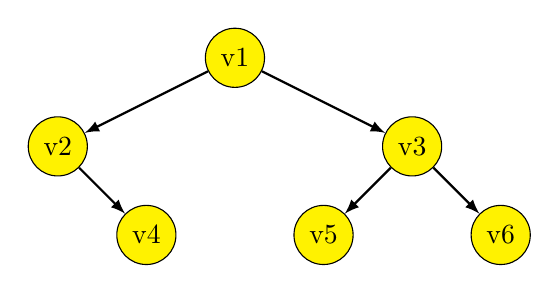
\begin{tikzpicture}[xscale=.5,yscale=.5]
% Styles (MODIFIABLES)
\tikzstyle{fleche}=[->,>=latex,thick]
\tikzstyle{noeud}=[fill=yellow,circle,draw]
\tikzstyle{feuille}=[fill=orange,circle,draw]
% Dimensions (MODIFIABLES)
\def\DistanceInterNiveaux{3}
\def\DistanceInterFeuilles{2}
% Dimensions calculées (NON MODIFIABLES)
\def\NiveauA{(-0)*\DistanceInterNiveaux}
\def\NiveauB{(-.75)*\DistanceInterNiveaux}
\def\NiveauC{(-1.5)*\DistanceInterNiveaux}
\def\NiveauD{(-2.25)*\DistanceInterNiveaux}
\def\InterFeuilles{(.75)*\DistanceInterFeuilles}
% Noeuds (MODIFIABLES : Styles et Coefficients d'InterFeuilles)
\node[noeud] (R) at ({(0)*\InterFeuilles},{\NiveauA}) {v1};
\node[noeud] (Ra) at ({(-3)*\InterFeuilles},{\NiveauB}) {v2};
\node[noeud] (Rb) at ({(3)*\InterFeuilles},{\NiveauB}) {v3};
\node[noeud] (Rab) at ({(-1.5)*\InterFeuilles},{\NiveauC}) {v4};
\node[noeud] (Rba) at ({(1.5)*\InterFeuilles},{\NiveauC}) {v5};
\node[noeud] (Rbb) at ({(4.5)*\InterFeuilles},{\NiveauC}) {v6};
% Arcs (MODIFIABLES : Styles)
\draw[fleche] (R)--(Ra);
\draw[fleche] (R)--(Rb);
\draw[fleche] (Ra)--(Rab);
\draw[fleche] (Rb)--(Rba);
\draw[fleche] (Rb)--(Rbb);
\end{tikzpicture}
\end{center}
Donner la liste des véhicules \code{v1}, \code{v2}, \code{v3}, \code{v4}, \code{v5}, \code{v6} triée dans l'ordre croissant de leur prix.
\item Recopier et compléter le code de la fonction récursive \code{contient} donnée ci-dessous, qui
prend en arguments un nombre \code{prix\_souhaite} de type \code{float} et un arbre binaire de recherche \code{abr} contenant des éléments de type \code{Veh} ordonnés selon leur prix estimé par la méthode \code{estim\_prix}. 

La fonction \code{contient(prix\_souhaite, abr)} renvoie \code{True} s'il existe un véhicule dans \code{abr} d'un prix estimé inférieur ou égal à \code{prix\_souhaite} et \code{False} sinon.

\pagebreak
\begin{Python*}
def contient(prix_souhaite, abr):
    if abr.est_vide():
        return False
    elif abr.get_v().estim_prix() <= ……… :
        return True 
    else:
        return contient( prix_souhaite , ……… ) 
\end{Python*}
\end{enumerate}
\end{enumerate}



























\newpage
\section*{Exercice 5}
\emph{Cet exercice porte sur les structures de données linéaires}

\medskip
Une méthode simple pour gérer l'ordonnancement des processus est d'exécuter les processus
en une seule fois et dans leur ordre d'arrivée.
\begin{enumerate}
\item Parmi les propositions suivantes, quelle est la structure de données la plus appropriée pour
mettre en œuvre le mode FIFO (First In First Out) ?
\begin{enumerate}
\item liste
\item dictionnaire
\item pile
\item file
\end{enumerate}
\item On choisit de stocker les données des processus en attente à l'aide d'une liste Python \code{lst}.
On dispose déjà d'une fonction \code{retirer(lst)} qui renvoie l'élément \code{lst[0]} puis le
supprime de la liste \code{lst}. Écrire en Python le code d'une fonction \code{ajouter(lst, proc)} qui
ajoute à la fin de la liste lst le nouveau processus en attente \code{proc}.
\end{enumerate}

On choisit maintenant d'implémenter une file \code{file} à l'aide d'un couple \code{(p1,p2)} où \code{p1} et \code{p2}
sont des piles. Ainsi \code{file[0]} et \code{file[1]} sont respectivement les piles \code{p1} et \code{p2}.
Pour enfiler un nouvel élément \code{elt} dans \code{file}, on l'empile dans \code{p1}.
Pour défiler \code{file}, deux cas se présentent.
\begin{itemize}
    \item La pile \code{p2} n'est pas vide : on dépile \code{p2}.
    \item La pile \code{p2} est vide : on dépile les éléments de \code{p1} en les empilant dans \code{p2} jusqu'à ce
    que \code{p1} soit vide, puis on dépile \code{p2}.
\end{itemize}
\begin{center}
    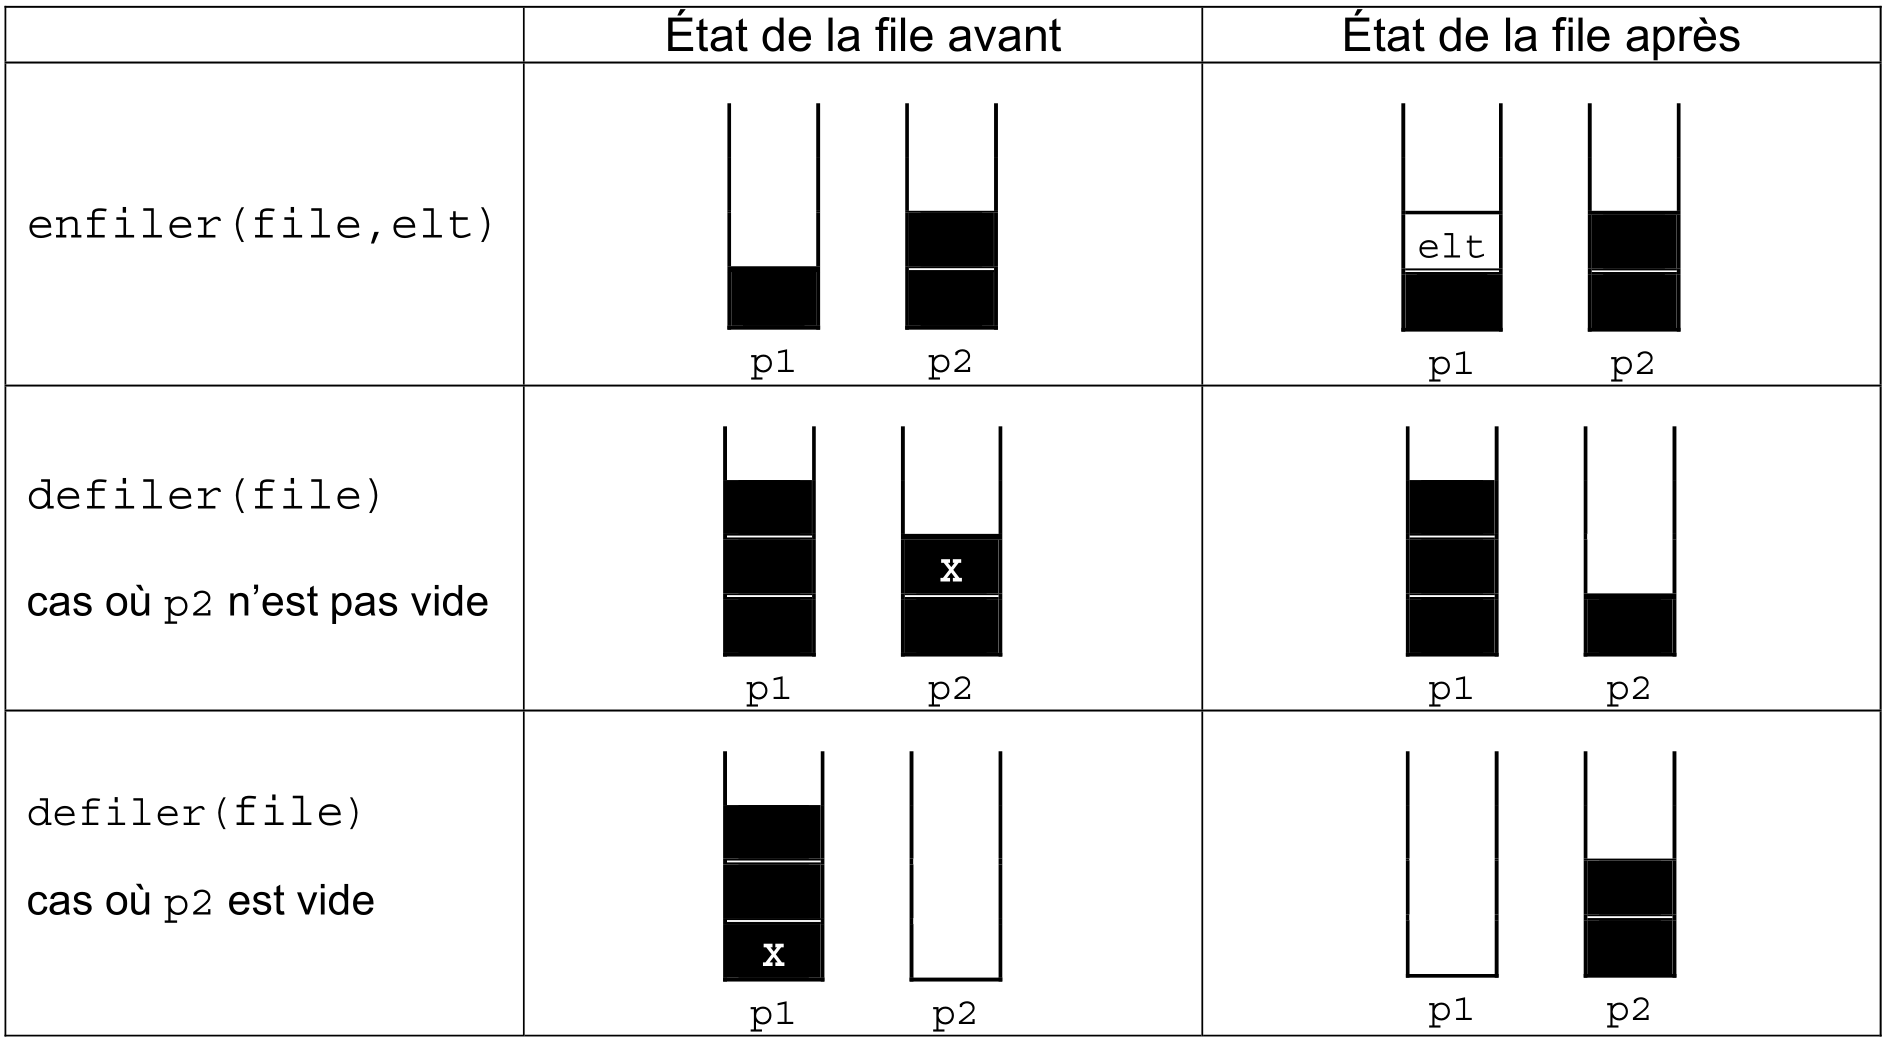
\includegraphics[width=\textwidth]{BacBlanc2Sujet2_NSI2122-img1.png}
    
    Illustration du fonctionnement des fonctions \code{enfiler} et \code{defiler}.
\end{center}

\newpage
\begin{enumerate}\setcounter{enumi}{2}
\item On considère la situation représentée ci-dessous.

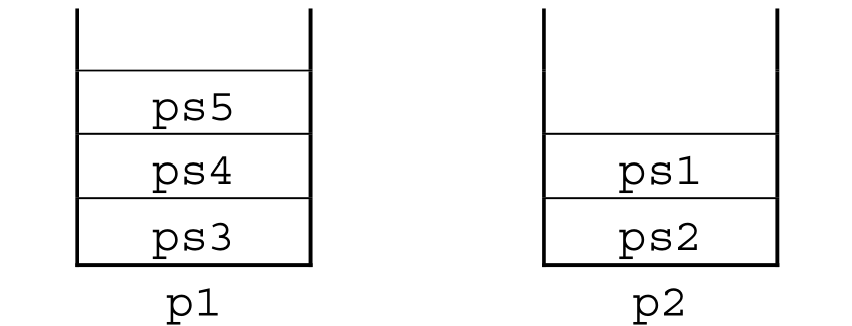
\includegraphics[width=0.4\textwidth]{BacBlanc2Sujet2_NSI2122-img2.png}

On exécute la séquence d'instructions suivante :
\begin{alltt}
enfiler(file,ps6)
defiler(file)
defiler(file)
defiler(file)
enfiler(file,ps7)
\end{alltt}
Représenter le contenu des deux piles (en précisant les éventuels éléments renvoyés) après chacune de ces instructions. 
\item On dispose des fonctions :
\begin{itemize}
    \item \code{empiler(p,elt)} qui empile l'élément \code{elt} dans la pile \code{p},
    \item \code{depiler(p)} qui renvoie le sommet de la pile \code{p} si \code{p} n'est pas vide et le
    supprime,
    \item \code{pile\_vide(p)} qui renvoie \code{True} si la pile \code{p} est vide, \code{False} si la pile \code{p} n'est pas vide.
\end{itemize}
et on veut les utiliser pour implémenter les fonctions dont on a observé le fonctionnement à la question précédente. 
\begin{enumerate}
    \item Écrire en Python une fonction \code{est\_vide(f)} qui prend en argument un couple de
    piles \code{f} et qui renvoie \code{True} si la file représentée par \code{f} est vide, \code{False} sinon.
    \item Écrire en Python une fonction \code{enfiler(f,elt)} qui prend en arguments un couple de
    piles \code{f} et un élément \code{elt} et qui ajoute \code{elt} en queue de la file représentée par \code{f}.
    \item Écrire en Python une fonction \code{defiler(f)} qui prend en argument un couple de piles \code{f}
    et qui renvoie l'élement en tête de la file représentée par \code{f} en le retirant.
\end{enumerate}
\item Au moyen des fonctions précédemment définies, écrire une fonction prenant comme argument une file \code{f} et renvoyant une file contenant les mêmes éléments que \code{f}, mais donnés dans l'ordre inverse. 
\end{enumerate}


\end{document}

